% Compile with XeLaTeX (Overleaf: Menu > Settings > Compiler > XeLaTeX).
% Gemini theme: https://github.com/anishathalye/gemini (fork: https://rev.cs.uchicago.edu/k4rtik/gemini-uccs)

\documentclass[final]{beamer}

% ====================
% Packages
% ====================

\usepackage[T1]{fontenc}
\usepackage{lmodern}
% COLM poster: 34 x 34 in = 86.36 x 86.36 cm
\usepackage[size=custom,width=86.36,height=86.36,scale=1.0]{beamerposter}
\usetheme{gemini}
\usecolortheme{stanford}
\usepackage{graphicx}
\usepackage{booktabs}
\usepackage{xcolor}
\usepackage{caption}
\usepackage{amsmath}

% ====================
% Colours: red and white title bar
% ====================
\setbeamercolor{headline}{bg=cardinalred, fg=white}
\setbeamercolor{headline title}{fg=white}
\setbeamercolor{headline author}{fg=white}
\setbeamercolor{headline institute}{fg=white}
\setbeamercolor{headline rule}{bg=darkred}
\setbeamerfont{headline title}{size=\LARGE,series=\bfseries}
\setbeamerfont{headline author}{size=\large}
\setbeamerfont{headline institute}{size=\normalsize}
% TL;DR box: red title bar, light warm-grey body (no blue)
\definecolor{warmgray}{RGB}{247, 244, 242}
\setbeamercolor{block title alerted}{fg=white,bg=cardinalred}
\setbeamercolor{block body alerted}{fg=black,bg=warmgray}
\definecolor{offc}{HTML}{f26b1d}
\definecolor{onc}{HTML}{0aa6c9}
\definecolor{ssdc}{HTML}{1f9e5c}
\newcommand{\off}{\textcolor{offc}{\textbf{off-policy}}}
\newcommand{\on}{\textcolor{onc}{\textbf{on-policy}}}
\newcommand{\ssd}{\textcolor{ssdc}{\textbf{SSD}}}
\newcommand{\hl}[1]{\textcolor{cardinalred}{\textbf{#1}}}

% ====================
% Fonts
% ====================
\setbeamerfont{block body}{size=\large}
\setbeamerfont{block title}{size=\Large}
\setbeamerfont{itemize/enumerate body}{size=\large}
\setbeamerfont{itemize/enumerate subbody}{size=\large}
\setbeamerfont{caption}{size=\normalsize}
\setbeamerfont{caption name}{size=\normalsize}
\captionsetup{font=normalsize,labelfont={normalsize,bf},skip=4pt}
\setbeamertemplate{caption label separator}{.\ }
\newcommand{\sub}[1]{\vspace{0.35em}{\large\bfseries\color{cardinalred}#1}\par\vspace{0.1em}}

% ====================
% Lengths: 3 columns
% ====================
% 4*\sepwidth + 3*\colwidth = \paperwidth  ->  4*0.02 + 3*0.3067 = 1
\newlength{\sepwidth}
\newlength{\colwidth}
\setlength{\sepwidth}{0.02\paperwidth}
\setlength{\colwidth}{0.3067\paperwidth}
\newcommand{\separatorcolumn}{\begin{column}{\sepwidth}\end{column}}

% ====================
% Title bar
% ====================
\title{Speculative Self-Distillation enables Efficient Knowledge Internalization}
\author{%
  Shayan Talaei*\inst{1} \and
  Agam Bhatia*\inst{1} \and
  Arshia Soltani Moakhar\inst{1} \and
  Jonas H\"ubotter\inst{2} \and
  Amin Saberi\inst{1} \and
  Azalia Mirhoseini\inst{1}
}
\institute{\inst{1}Stanford University \qquad \inst{2}ETH Z\"urich \qquad *Equal contribution}

\logoleft{%
  \begin{minipage}{8cm}\centering
    
\includegraphics[height=2.8cm]{figures/logo_stanford_white.pdf}\\[0.9cm]
    
\includegraphics[height=1.7cm]{figures/logo_eth_white.pdf}
  \end{minipage}}
\logoright{%
  \begin{minipage}{8cm}\centering
    
\includegraphics[height=5.6cm]{figures/qr_paper.pdf}\\[0.25cm]
    {\large\bfseries\color{white} PAPER}
  \end{minipage}}

% ====================
% Body
% ====================
\begin{document}
\begin{frame}[t]
\begin{columns}[t]
\separatorcolumn

% =================================== column 1 ===================================
\begin{column}{\colwidth}

  \begin{alertblock}{TL;DR}
    \vspace{0.5em}\centering
    \begin{minipage}{0.93\linewidth}\large\raggedright
    We teach a language model a document by \textbf{self-distillation}: the model reads the document and acts as a
    teacher for itself without it. \ssd{} lets the \textbf{student write each training rollout} and lets the teacher
    \textbf{take over only at tokens where the two disagree}. It reaches \on{} accuracy with
    \textbf{45\% fewer supervised tokens} on average and \textbf{forgets less} of the model's general ability.
    \end{minipage}
    \vspace{0.6em}
  \end{alertblock}

  \begin{block}{Background and Motivation}
    \sub{Knowledge in the weights}
    \begin{itemize}
      \item Models are often needed on knowledge \hl{absent from pretraining}: private documents, facts that changed
            after the cutoff, specialised domains.
      \item Putting it in the prompt costs context and compute \hl{on every query}, and in-context evidence is not
            always used reliably. Training it into the weights is paid once.
    \end{itemize}
    \sub{Self-distillation}
    \begin{itemize}
      \item \textbf{Teacher} $\pi_T(\cdot\mid x, C)$: the model with the document $C$ in context.
            \textbf{Student} $\pi_\theta(\cdot\mid x)$: the same model without it.
      \item The student matches the teacher token by token along rollouts $y$:
    \end{itemize}
    \vspace{-0.4em}
    \[ \mathcal{L}(\theta)=\mathbb{E}_{y\sim\pi_{\text{gen}}}\Big[\tfrac{1}{|y|}\textstyle\sum_t
       D\big(\pi_T(\cdot\mid x,C,y_{<t})\,\|\,\pi_\theta(\cdot\mid x,y_{<t})\big)\Big] \]
    \vspace{-0.6em}
    \begin{itemize}
      \item Methods differ only in \hl{who writes the rollout}, $\pi_{\text{gen}}$:
        \begin{itemize}
          \item \off{} (teacher writes): fast, but trains on text the student would not produce.
          \item \on{} (student writes, e.g.\ SDFT): matches test-time behaviour, but slow.
        \end{itemize}
    \end{itemize}
  \end{block}

  \begin{block}{Why On-Policy Training Is Slow}
    \centering
    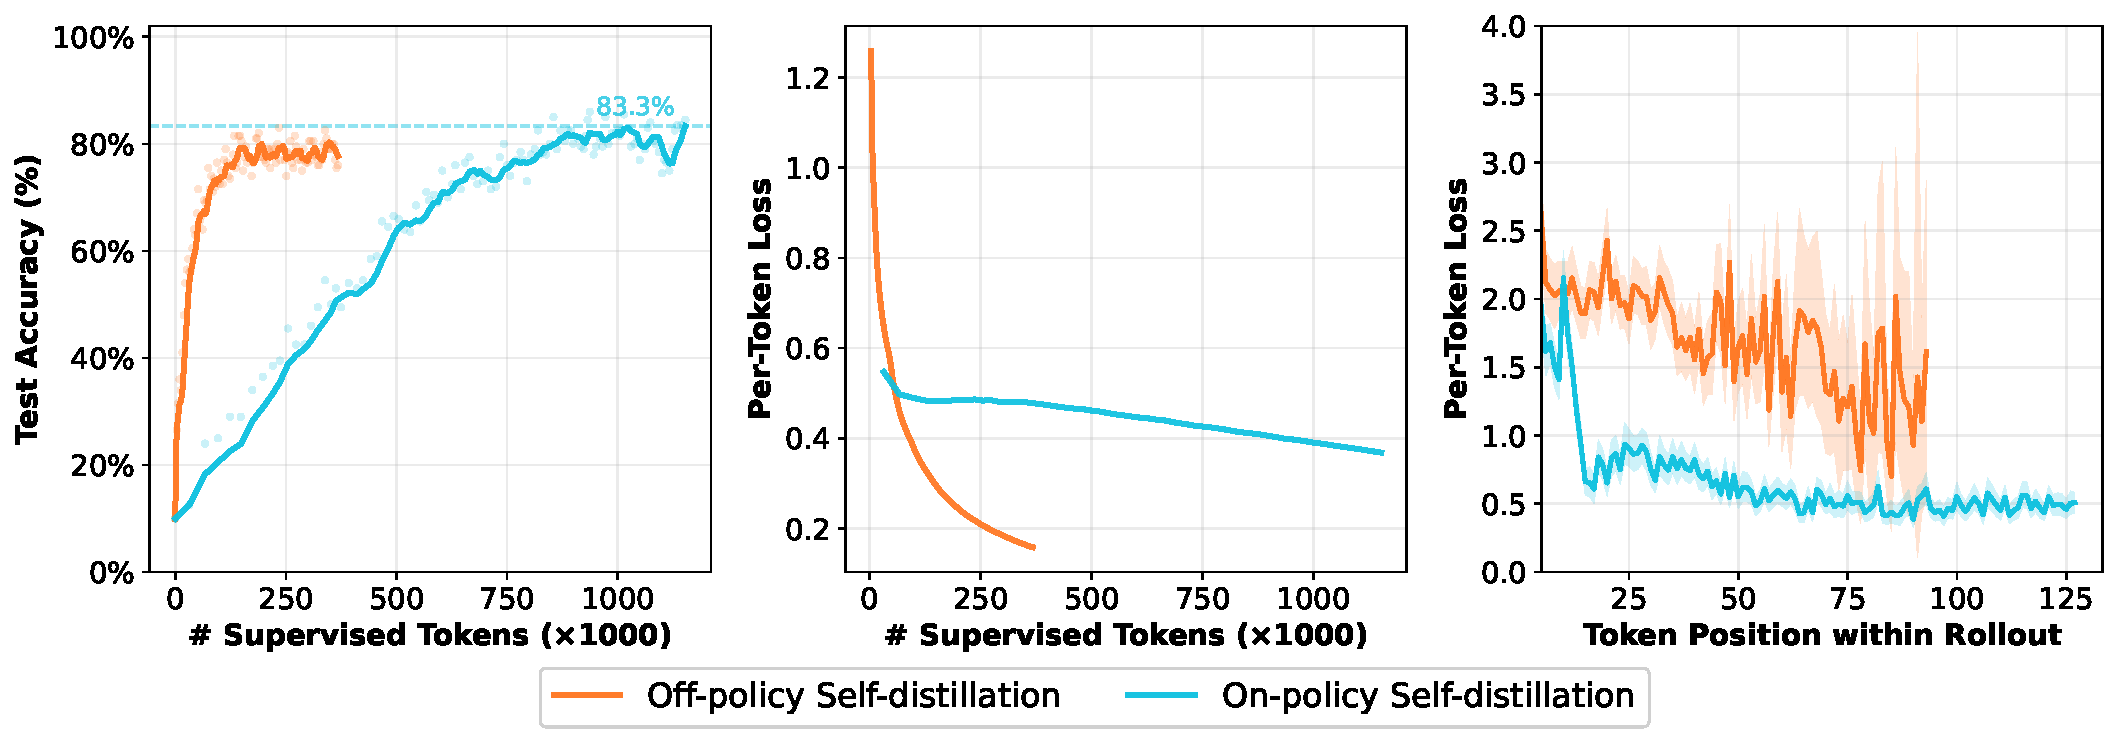
\includegraphics[width=\textwidth]{figures/signal_panel.pdf}
    \captionof{figure}{Wikipedia task. Left: accuracy. Middle: per-token loss during training. Right: per-token loss by
      position within a rollout.}
    \raggedright
    \begin{itemize}
      \item The per-token loss measures how much the student can learn from a token; we call it the \hl{signal}.
      \item \off{} converges \textbf{$\sim$5$\times$ faster} but plateaus lower.
      \item Along \on{} rollouts the signal \hl{collapses after a few tokens}: the student drifts away from the document,
            and the teacher, conditioned on that prefix, has little left to correct.
    \end{itemize}
  \end{block}

\end{column}
\separatorcolumn

% =================================== column 2 ===================================
\begin{column}{\colwidth}

  \begin{block}{Speculative Self-Distillation (SSD)}
    \centering
    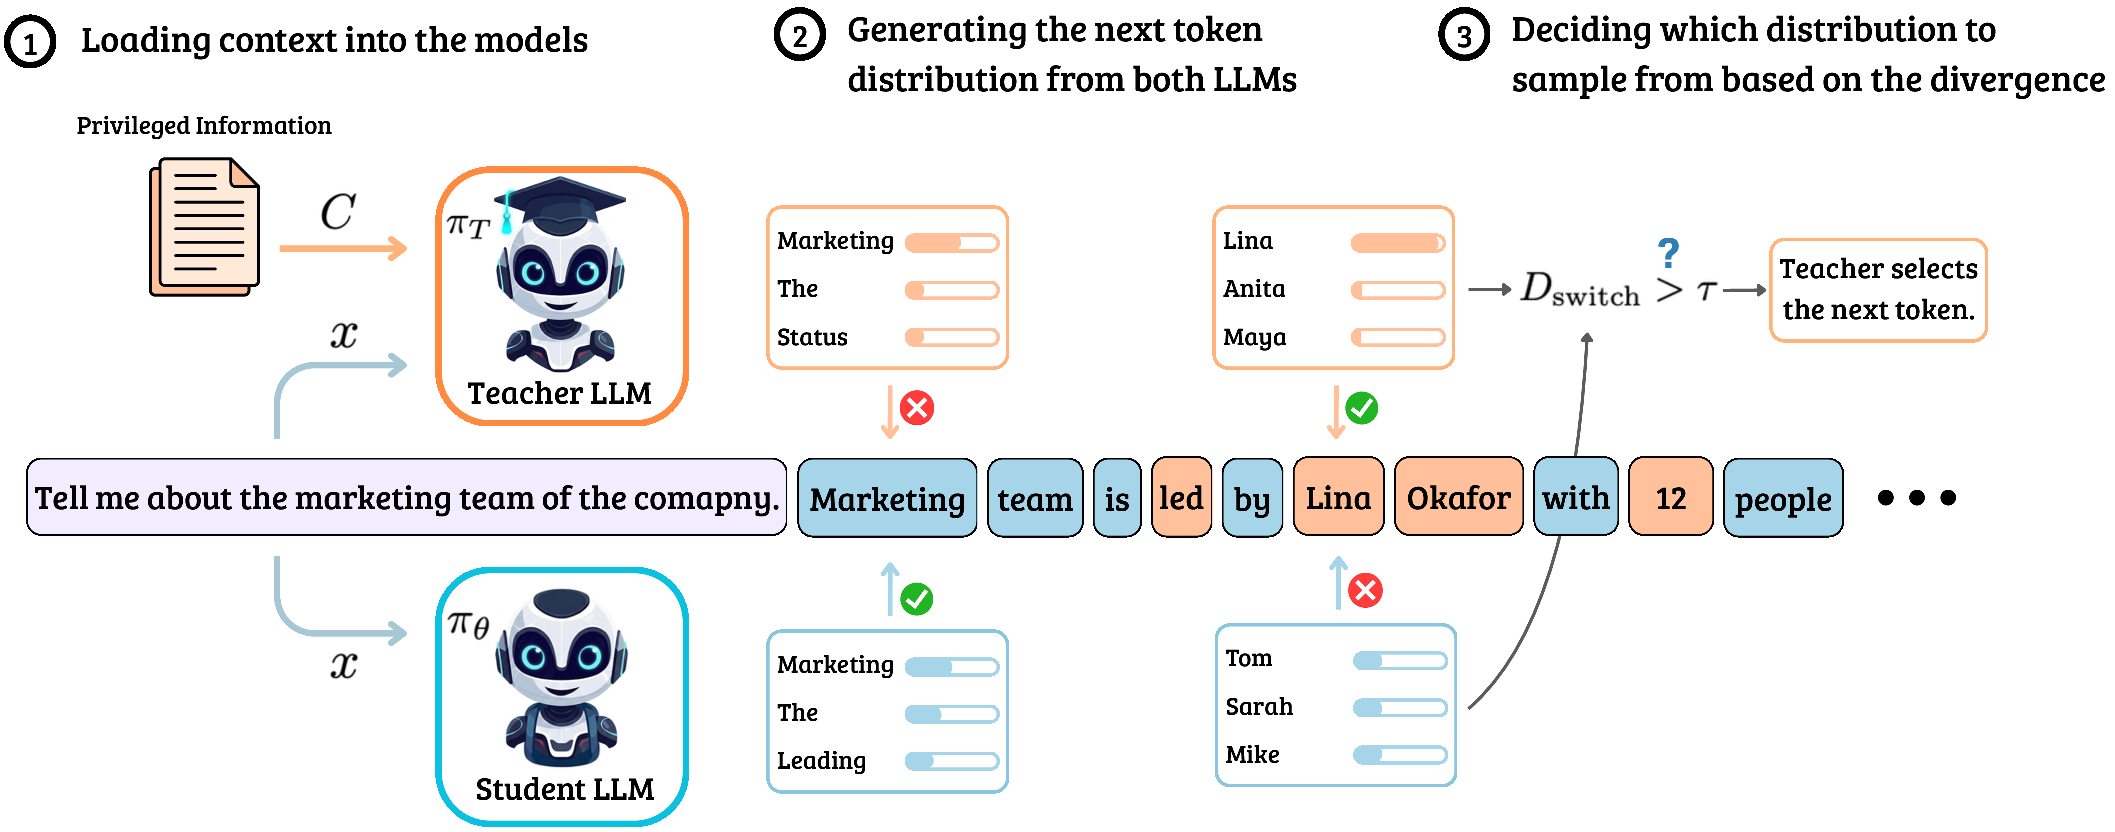
\includegraphics[width=\textwidth]{figures/main_figure.pdf}
    \captionof{figure}{The SSD decoding loop. Both models propose a next-token distribution; when their divergence
      exceeds $\tau$ the teacher picks the token, otherwise the student does.}
    \raggedright
    \begin{itemize}
      \item The \textbf{student generates by default}. At every position we compute
            $\delta_t = D_{\text{switch}}(\pi_\theta \,\|\, \pi_T)$.
      \item If $\delta_t > \tau$ the position is an \hl{inflection token} and the \textbf{teacher samples} it.
      \item Every position is supervised with the same loss $D_{\text{loss}}$; only the rollout changes.
      \item One knob: $\tau\!\to\!0$ recovers \off{}, $\tau\!\to\!\infty$ recovers \on{}.
            With JSD as $D_{\text{switch}}$ the divergence is at most $\ln 2$.
    \end{itemize}
  \end{block}

  \begin{block}{Inflection Tokens}
    \centering
    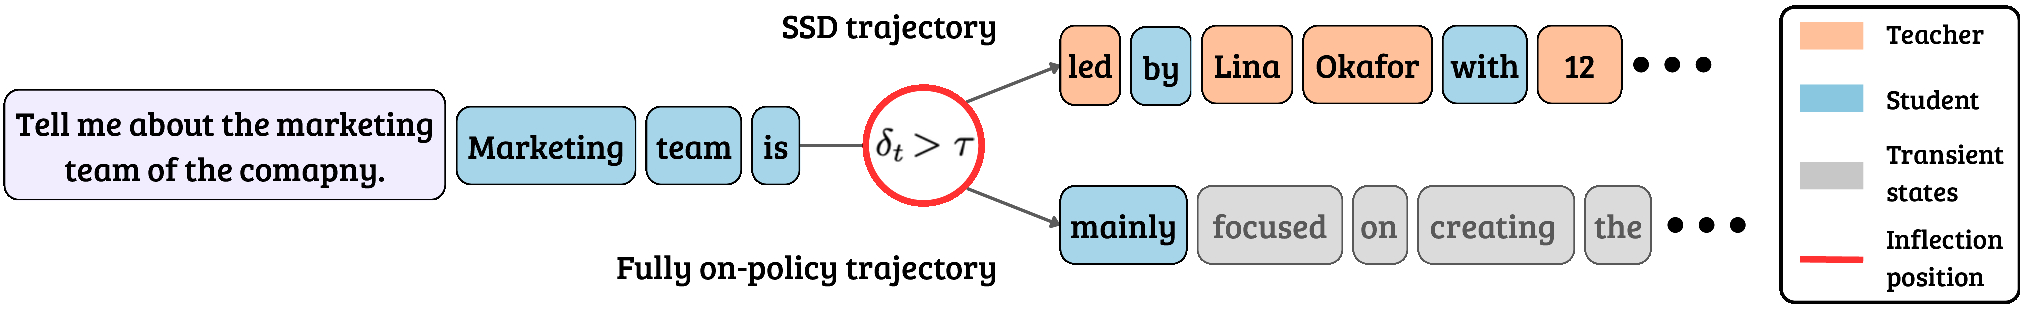
\includegraphics[width=\textwidth]{figures/influence_positions.pdf}
    \captionof{figure}{An example rollout. SSD lets the teacher write at the inflection position; on-policy keeps the
      student's token and continues into transient states.}
    \raggedright
    \begin{itemize}
      \item Student and teacher agree on ``Marketing team is'', then diverge: the teacher has read the memo
            (``led by Lina Okafor''), the student has not (``mainly focused on \ldots'').
      \item After an \on{} inflection, later tokens are \hl{transient states}: the update moves the student away from
            ``mainly'', so it will rarely visit them again and supervision on them is largely wasted.
      \item \ssd{} keeps the rollout on the informative path while staying close to the student elsewhere.
    \end{itemize}
  \end{block}

  \begin{block}{Experimental Setup}
    \begin{itemize}
      \item \textbf{Model}: Qwen3-4B-Instruct as both student and teacher; teacher frozen at the initial weights.
      \item \textbf{Tasks} (closed-book QA): \textbf{Company Memo} (synthetic private document), \textbf{Wikipedia}
            (article after the training cutoff), \textbf{Science Q\&A} (SciKnowEval Chemistry L-3).
      \item \textbf{Baselines}: \off{} SFT and FKL on teacher rollouts; \on{} SDFT.
      \item \textbf{Cost}: supervised tokens, the number of positions the loss is computed on (roughly proportional
            to compute).
    \end{itemize}
  \end{block}

\end{column}
\separatorcolumn

% =================================== column 3 ===================================
\begin{column}{\colwidth}

  \begin{block}{Results}
    \centering
    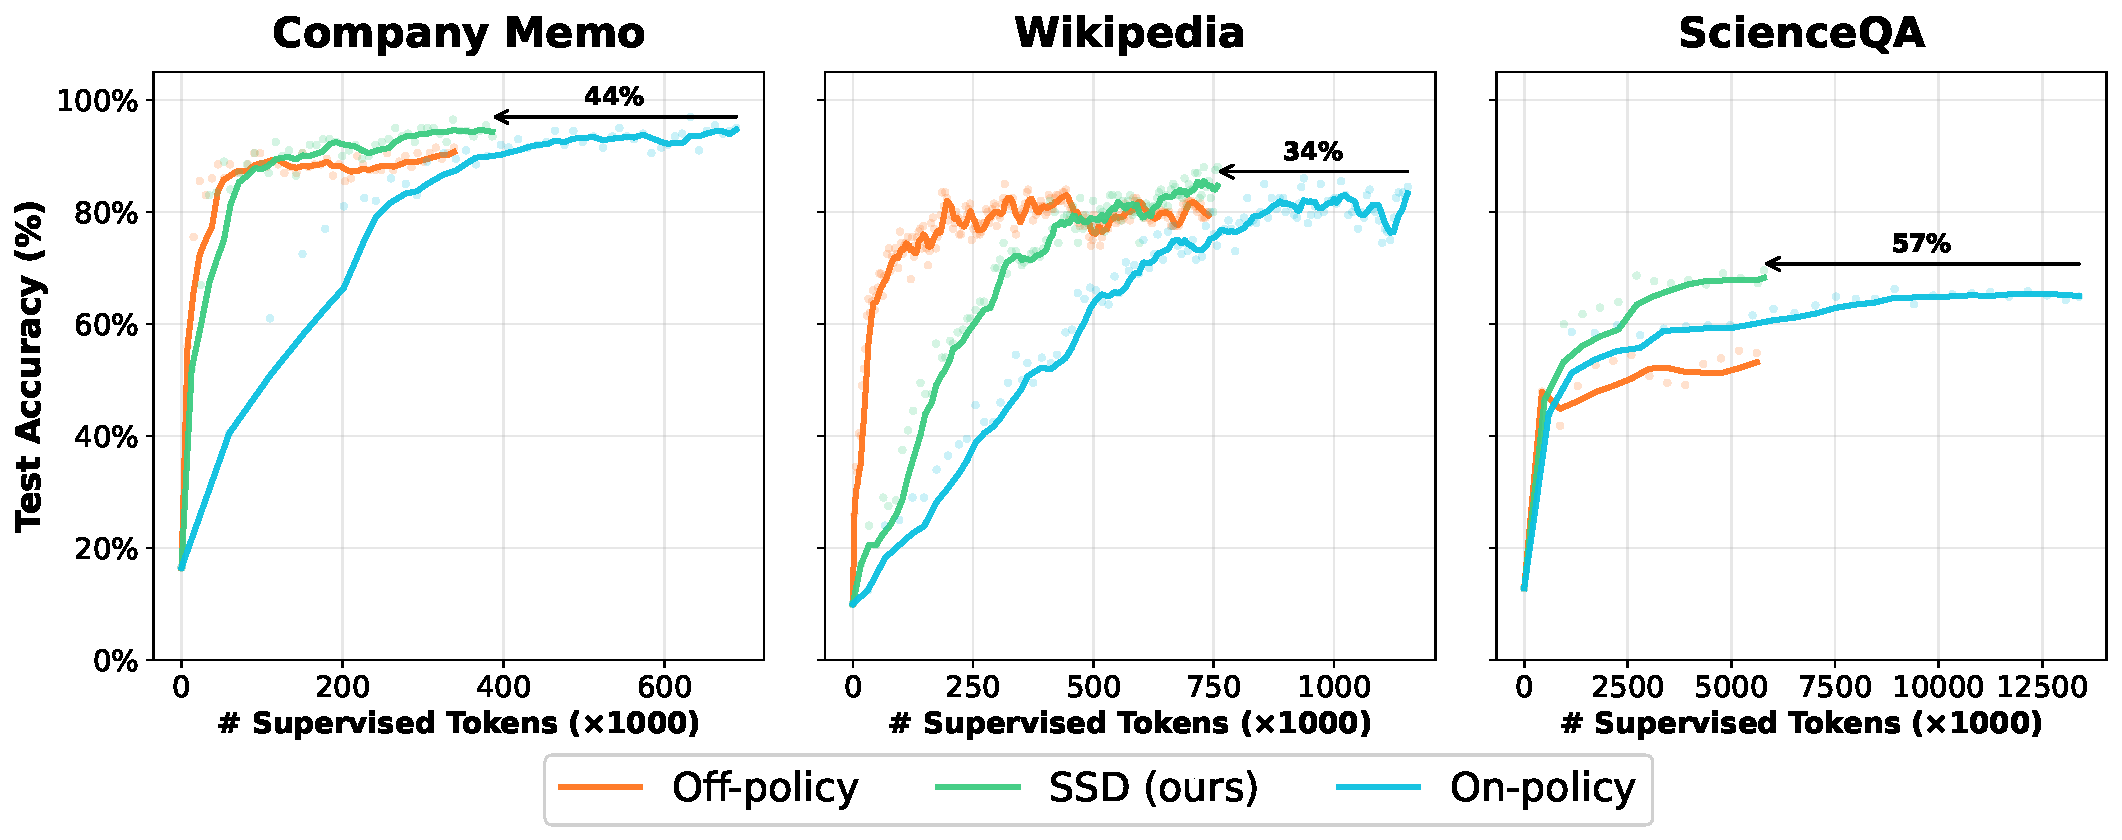
\includegraphics[width=\textwidth]{figures/figure_1_smoothed.pdf}
    \captionof{figure}{Test accuracy against supervised tokens on the three tasks.}
    \raggedright
    \begin{itemize}
      \item \ssd{} rises with \off{}'s early slope and continues to the \on{} plateau, using
            \hl{44\%, 34\% and 57\% fewer supervised tokens} than \on{}.
      \item On Science Q\&A it ends about \textbf{3 points above} \on{} and \textbf{15 above} \off{}.
    \end{itemize}
  \end{block}

  \begin{block}{Choosing $\tau$, and a Built-in Curriculum}
    \begin{columns}[t]
      \begin{column}{0.49\textwidth}
        \centering
        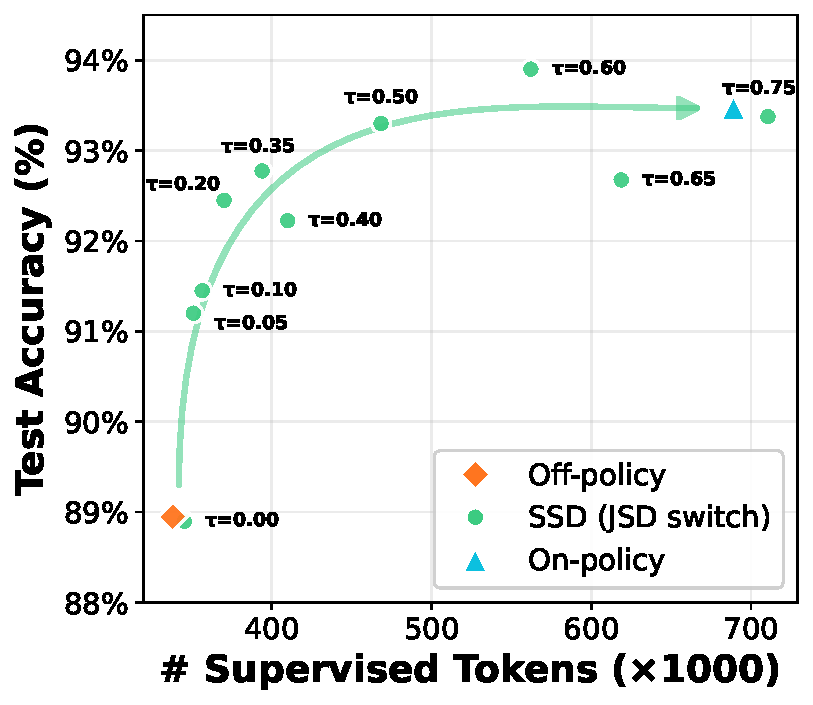
\includegraphics[width=\textwidth]{figures/tau_frontier.pdf}
        \captionof{figure}{Accuracy vs.\ cost across $\tau$ (Company Memo).}
      \end{column}
      \begin{column}{0.49\textwidth}
        \centering
        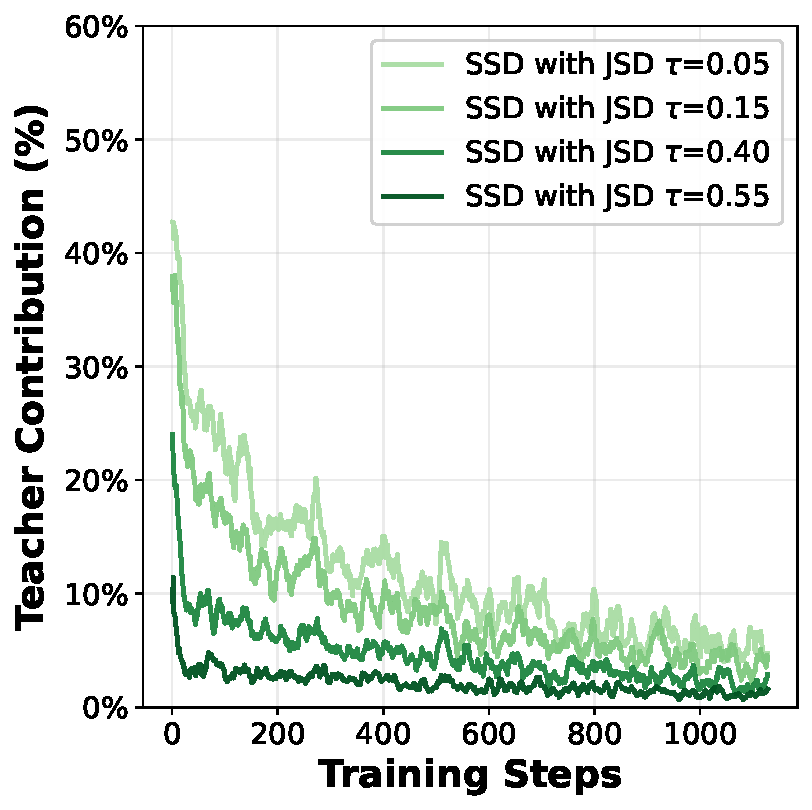
\includegraphics[width=\textwidth]{figures/teacher_contribution.pdf}
        \captionof{figure}{Share of rollout tokens written by the teacher.}
      \end{column}
    \end{columns}
    \begin{itemize}
      \item Sweeping $\tau$ traces a \hl{Pareto frontier}; $\tau \in [0.2, 0.5]$ (JSD) works well.
      \item The teacher writes up to 40\% of tokens early on; its share falls as the student learns, so training
            becomes \on{} \hl{without a schedule}.
    \end{itemize}
  \end{block}

  \begin{block}{Less Forgetting}
    \vspace{0.3em}
    \begin{columns}[T]
      \begin{column}{0.40\textwidth}
        Qwen2.5-7B on SciKnowEval chemistry, scored on six general benchmarks.\\[0.4em]
        \ssd{} has the best SciQA (\textbf{71.6}) and the smallest drop (\hl{$-$1.4} vs $-$4.5 for SDFT).
      \end{column}
      \begin{column}{0.58\textwidth}
        \centering
        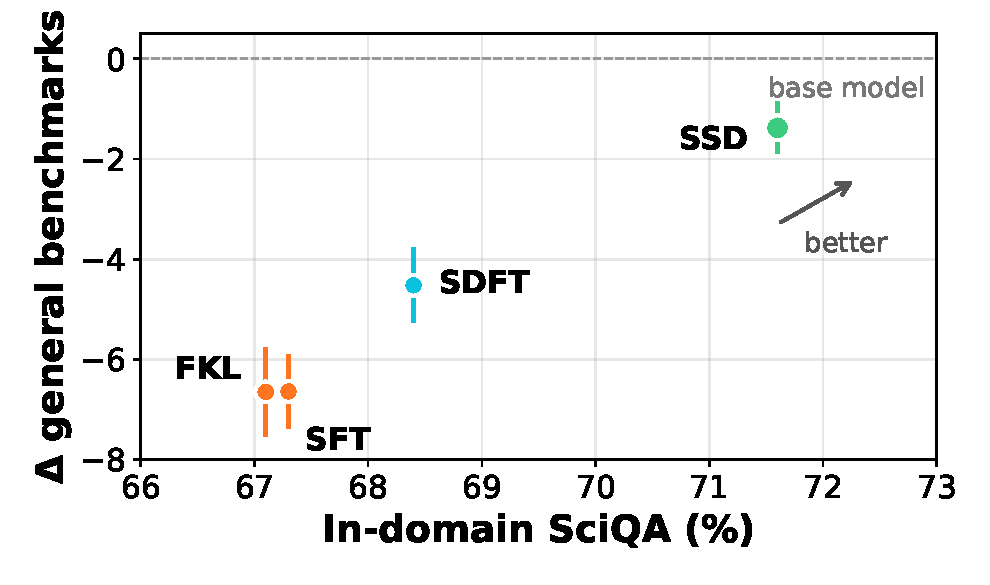
\includegraphics[width=\textwidth]{figures/forgetting.pdf}
      \end{column}
    \end{columns}
  \end{block}

  \begin{block}{Conclusion}
    \begin{itemize}
      \item The useful signal in self-distillation is concentrated at the few tokens where the document changes the
            prediction.
      \item Letting the teacher write only there gives \on{} accuracy at close to \off{} cost, with less forgetting.
    \end{itemize}
  \end{block}

\end{column}
\separatorcolumn
\end{columns}
\end{frame}
\end{document}
